\documentclass[tikz,dvisvgm]{standalone}

\usetikzlibrary {positioning,arrows.meta,fit,backgrounds}

\pgfdeclarelayer{coders}
\pgfdeclarelayer{layers}
\pgfdeclarelayer{containers}
\pgfsetlayers{coders,layers,containers,main}

\begin{document}
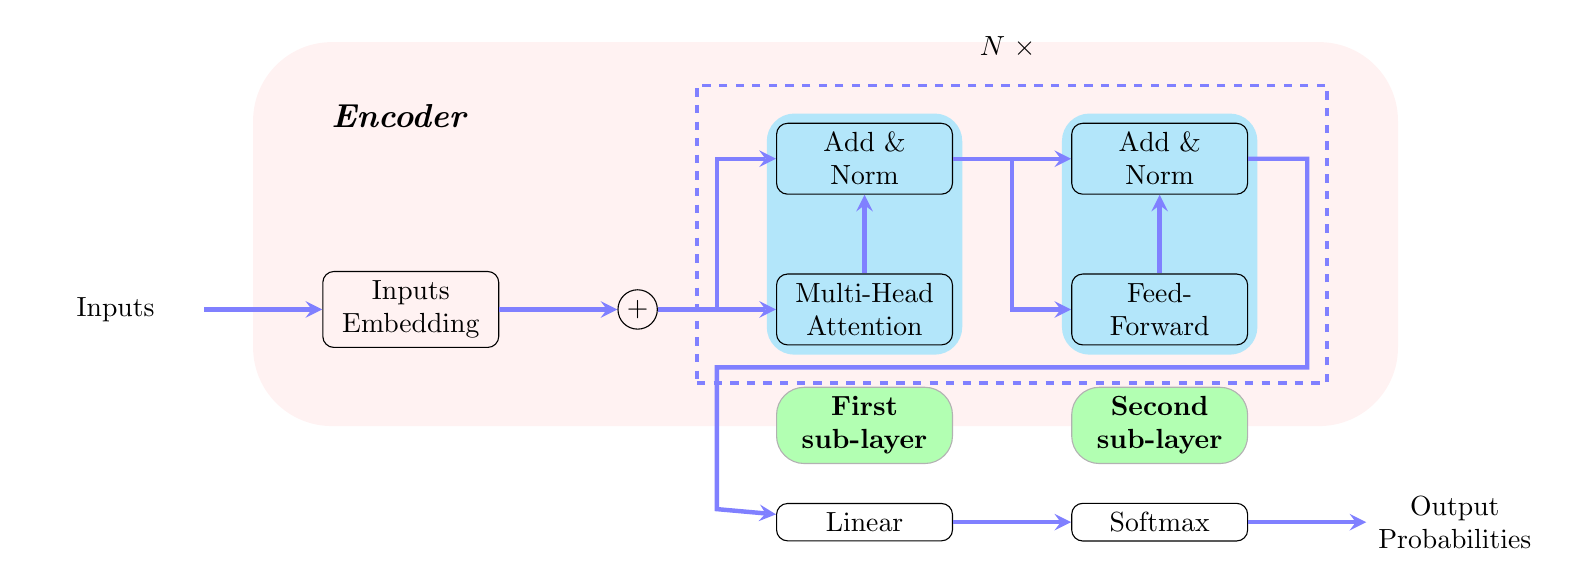
\begin{tikzpicture}[
    every text node part/.style={align=center,text width=2cm,},
    nn/.style = {draw,rectangle,rounded corners},
    arr/.style = {draw=blue!50, ultra thick},-stealth,
    plus/.style= {draw,circle,inner sep=0pt,minimum size=0.5cm,text width=0cm,align=center},
    conn/.style = {draw=blue!50, ultra thick},
    layer/.style = {fill=cyan!30, rounded corners=10pt},
    container/.style = {draw=blue!50, dashed, very thick, inner xsep=25pt, inner ysep=10pt},
    coder/.style = {inner xsep=25pt, inner ysep=15pt, rounded corners = 1cm},
    layertext/.style = {fill=green!30,draw=black!30,rectangle,rounded corners=10pt,font=\bfseries},
    node distance = 1cm and 1.5cm,
  ]

  \node (inputs) {Inputs};
  \node [nn,right= of inputs] (inputs-embedding) {Inputs \\ Embedding};
  \node [plus, right= of inputs-embedding] (plus) {};
  \node at (plus) {+};
  \path[arr] (inputs) to (inputs-embedding);
  \path[arr] (inputs-embedding) to (plus);

  \node [nn,right= of plus] (multi-head) {Multi-Head \\ Attention};
  \node [nn,above= of multi-head] (addnorm1) {Add \& Norm};
  \begin{pgfonlayer}{layers}
    \node [layer,fit=(multi-head) (addnorm1)] (sublayer1) {};
    \node [layertext,below=0.4cm of sublayer1] (firstsublab) {First sub-layer};
  \end{pgfonlayer}

  \path[arr] (multi-head) to (addnorm1);
  \coordinate[right=0.75cm of plus] (aux);
  \path[arr] (plus) to (multi-head);
  \path[arr] (aux) |- (addnorm1);

  \node [nn,right= of addnorm1] (addnorm2) {Add \& Norm};
  \node [nn] (feed-forward) at (addnorm2 |- multi-head) {Feed-Forward};

  \begin{pgfonlayer}{layers}
    \node [layer,fit=(feed-forward) (addnorm2)] (sublayer2) {};
    \node [layertext] at (sublayer2 |- firstsublab) {Second sub-layer};
  \end{pgfonlayer}

  \path[arr] (feed-forward) to (addnorm2);
  \coordinate[right=0.75cm of addnorm1] (aux2);
  \path[arr] (addnorm1) to (addnorm2);
  \path[arr] (aux2) |- (feed-forward);

  \begin{pgfonlayer}{containers}
    \node [container, fit=(sublayer1) (sublayer2)] (encoder) {};
    \node [above=0.2cm of encoder] (ntimes) {$N \times{}$};
  \end{pgfonlayer}

  \begin{pgfonlayer}{coders}
    \node [fill=red!5,coder, fit=(encoder) (plus) (inputs-embedding)] (encoder-container) {};
    \node [left=-3cm of encoder-container,yshift=1.5cm] (encoderlab) {\large \textbf{\textit{Encoder}}};
  \end{pgfonlayer}

  \node [nn,below=2cm of multi-head] (linear) {Linear};
  \node [nn,right= of linear] (softmax) {Softmax};
  \node [right= of softmax] (proba) {Output Probabilities};

  \coordinate[right=0.75cm of addnorm2] (aux6);
  \coordinate [below=2.65cm of aux6] (aux7);
  \coordinate (aux8) at (aux |- aux7);
  \coordinate [below=1.8cm of aux8] (aux9);

  \draw [conn] (addnorm2) to (aux6) to (aux7) to (aux8) to (aux9) to (linear);

  \path[arr] (linear) to (softmax);
  \path[arr] (softmax) to (proba);
\end{tikzpicture}

\end{document}